\documentclass[a4paper,12pt]{article}
\usepackage{amsmath,amssymb,amsfonts,amsthm}
\usepackage{tikz}
\usepackage[utf8x]{inputenc}
\usepackage[T2A]{fontenc} 
\usepackage[russian]{babel}
\usepackage{cmap} 
\usepackage{ gensymb }
% Так ссылки в PDF будут активны
\usepackage[unicode]{hyperref}
\usepackage{ textcomp }
\usepackage{indentfirst}
\usepackage[version=3]{mhchem}

% вы сможете вставлять картинки командой \includegraphics[width=0.7\textwidth]{ИМЯ ФАЙЛА}
% получается подключать, как минимум, файлы .pdf, .jpg, .png.
\usepackage{graphicx}
% Если вы хотите явно указать поля:
\usepackage[margin=1in]{geometry}
% Или если вы хотите задать поля менее явно (чем больше DIV, тем больше места под текст):
% \usepackage[DIV=10]{typearea}

\usepackage{fancyhdr}

\newcommand{\bbR}{\mathbb R}%теперь вместо длинной команды \mathbb R (множество вещественных чисел) можно писать короткую запись \bbR. Вместо \bbR вы можете вписать любую строчку букв, которая начинается с '\'.
\newcommand{\eps}{\varepsilon}
\newcommand{\bbN}{\mathbb N}
\newcommand{\dif}{\mathrm{d}}

\newtheorem{Def}{Определение}


\pagestyle{fancy}
\makeatletter % сделать "@" "буквой", а не "спецсимволом" - можно использовать "служебные" команды, содержащие @ в названии
\fancyhead[L]{\footnotesize }%Это будет написано вверху страницы слева
\fancyhead[R]{\footnotesize ФУПМ МФТИ}
\fancyfoot[L]{\footnotesize \@author}%имя автора будет написано внизу страницы слева
\fancyfoot[R]{\thepage}%номер страницы —- внизу справа
\fancyfoot[C]{}%по центру внизу страницы пусто

\renewcommand{\maketitle}{%
	\noindent{\bfseries\scshape\large\@title\ \mdseries\upshape}\par
	\noindent {\large\itshape\@author}
	\vskip 2ex}
\makeatother
\def\dd#1#2{\frac{\partial#1}{\partial#2}}


\title{1.1 \\ Экспериментальная проверка уравнения Эйнштейна для фотоэффекта и определение постоянной Планка}
\author{Северилов Павел, 674} 
\date{1 декабря 2018 г.}

\begin{document}
	\maketitle
	\section*{Теория}
		Явление внешнего фотоэлектрического эффекта заключается в испускании электронов фотокадом. При столкновении фотона с энергией $\hbar\omega$ и импульсом $\dfrac{\hbar\omega}{c}$ с электроном фотокада энергия фотона полностью передается электрону и фотон прекращает свое существование. Соотношение энергий при столкновении описывается следующим соотношением: 
		\begin{equation}
			\hbar \omega = E_{max} + W,
		\end{equation}
		где $E_{max}$ -- максимальная кинетическая энергия электрона после выхода из фотокатода, $W$ -- работа выхода электрона из катода.
		
		Для измерения энергии вылетевших фотоэлектронов устанавливают второй электрод c задерживающим($V < 0$) или ускоряющим потенциалом($V > 0$).
		\begin{center}
			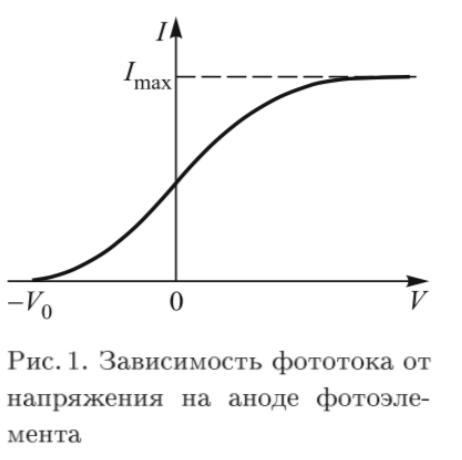
\includegraphics[width = 69 mm]{t1}
		\end{center}
		Максимальная кинетическая энергия $E_{max}$ электрона связана с запирающим потенцилом соотношением $E_{max} = eV_0$. И отсюда следует формула Эйнштейна для фотоэффекта:
		\begin{equation}
			eV_0 = \hbar\omega - W.
		\end{equation}
		Рассмотрим проблему нахождения максимальной кинетической энергии электронов $E_0$. Согласно квантовой механике, энергия частицы, находящиеся в потенциальной яме может принимать только дискретный набор значений. Для электронов говорят не об уровнях энергии, но об образовании зоны разрешенных значений энергии электронов в металле. Спин(угловой момент) электрона равен $1/2$, такие частицы называют фермионами, они подчиняются \textbf{принципу Паули: в одном квантовом состоянии находятся не более двух электронов}. Отсюда следует, что электроны проводимости не будут находиться на дне ямы, но заполнят все разрешенные уровни энергии от $0$ до $E+_F$ -- энергии Ферми, которая определяется концентрацией электронов. 
		
		При переходе электрона из металла в металле образуется <<симметричный>> заряд внутри металла, который притягивает электрон c силой $\dfrac{e^2}{4x^2}$. Суммируя работу получаем энергию $W$ нужную для вылета электрона на  величину порядка межатомных состояний.
		
		\begin{figure}[h]
				\begin{minipage}[h]{0.6\linewidth}
					\center{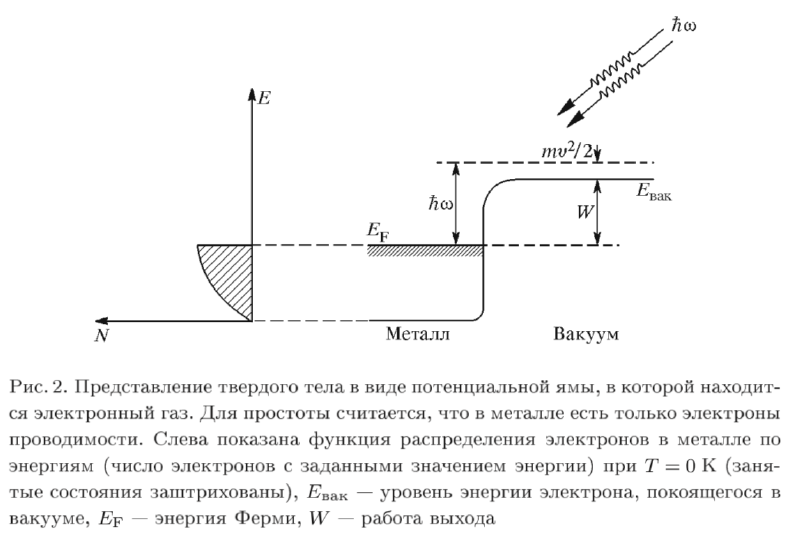
\includegraphics[width=1.5\linewidth]{t2}}
				\end{minipage}
				\hfill
				\hfill
				\begin{minipage}[h]{0.6\linewidth}
					\center{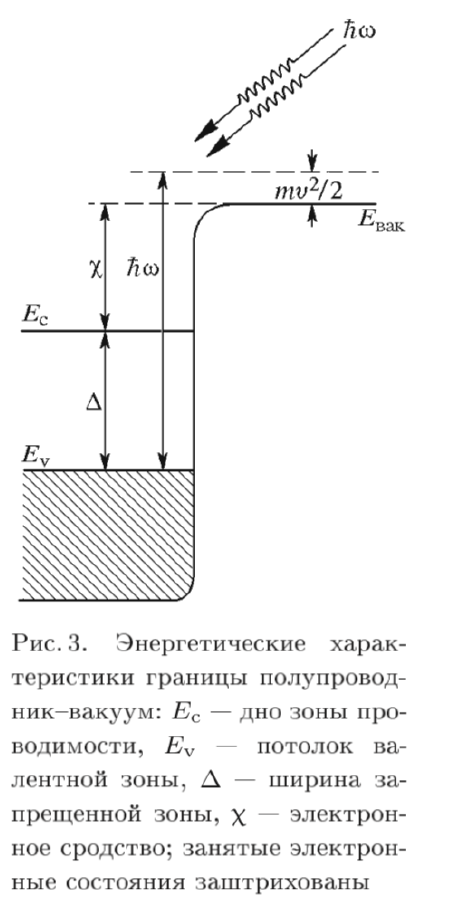
\includegraphics[width=0.5\linewidth]{t3} }
				\end{minipage}
			\end{figure}
		Распределение электронов в полупроводниках сильно отличается от распределения электронов в металлах: при нуле температур в полупроводниках внешние валентные электроны полностью заполняют зону разрешенных значений энергии, а в зоне проводимости их нет.
		
		
		Основные характеристики фотоэмиссии:
		\begin{enumerate}
			\item Ширина запрещенной зоны $\Delta$ -- разность энергий между потолком валентной зоны $E_v$ и дном зоны проводимости $E_c$.
			\item Электронное средство $\chi$ -- разность между краем зоны проводимости $E_c$ и уровнем энергии $E_{\text{вак}}$.
			\item Квантовый выход -- число эмитированных поверхностью вещества электронов, делённое на число падающих на поверхность фотонов.
		\end{enumerate}
		Для того чтобы свет мог выбить электрон из полупроводника минимальная энергия кванта должна превысить пороговое значение: 
		\begin{equation}
			W = \hbar\omega_{min} = \Delta + \chi
		\end{equation}
		\newpage
		\begin{center}
			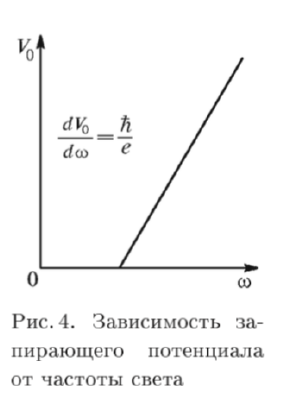
\includegraphics[width = 40 mm]{t4}
		\end{center}
		Для того, чтобы определить величину запирающего напряжения нам надо правильно экстраполировать получаемую токовую зависимость к нулю нам надо узнать функциональную зависимость $I(V)$. Расчет ддя плоского катода дает зависимость 
		\begin{equation}
			\sqrt{I} \propto (V_0 - V).
		\end{equation}
		В работе изучается зависимость фототока из фотоэлемента от величины потенциала $V$ для разных частот света $\omega$. Для этого строится зависимость $V_0(w)$: 
		\begin{equation}
			V_0(\omega) = \dfrac{\hbar\omega - W}{e}.
		\end{equation}
		Потенциал запирания линейно зависит от частоты света $\omega$, поэтому по наклону прямой можно найти постоянную Планка:
		\begin{equation}
			\dfrac{dV_0}{d\omega} = \dfrac{\hbar}{e}.
		\end{equation}
	%	\newpage
		
		\section*{Экспериментальная установка}
		Чувствительность ФЭ лежит в области от $300$ до $800$ нм.
		\begin{center}
			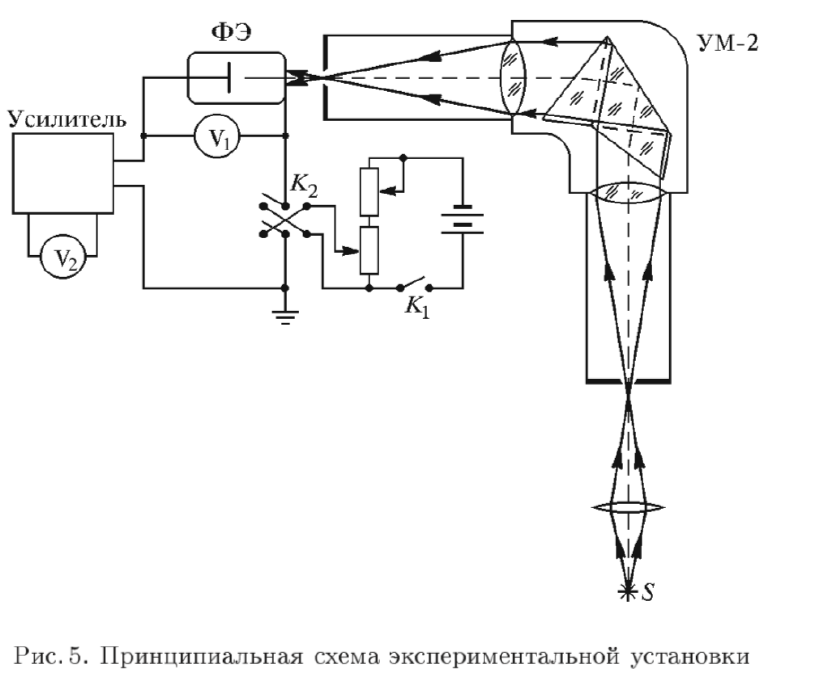
\includegraphics[width = 80 mm]{ust}
		\end{center}
		\section*{Результаты работы}
		
			Проведем все необходимые для проведения эксперимента мероприятия: включим блок питания, произведем градуировку монохроматора, заменим окуляр. Добьемся яркого света на входной щели монохроматора, её ширина примерно 0.3 мм. C помощью потенциометров <<Грубо>> и <<Плавно>> исследуем \textbf{зависимость показаний тока от величины тормозящего потенциала}.
			При градуировке запишем некоторые точки, получим прямую градуировки:
			\begin{center}
				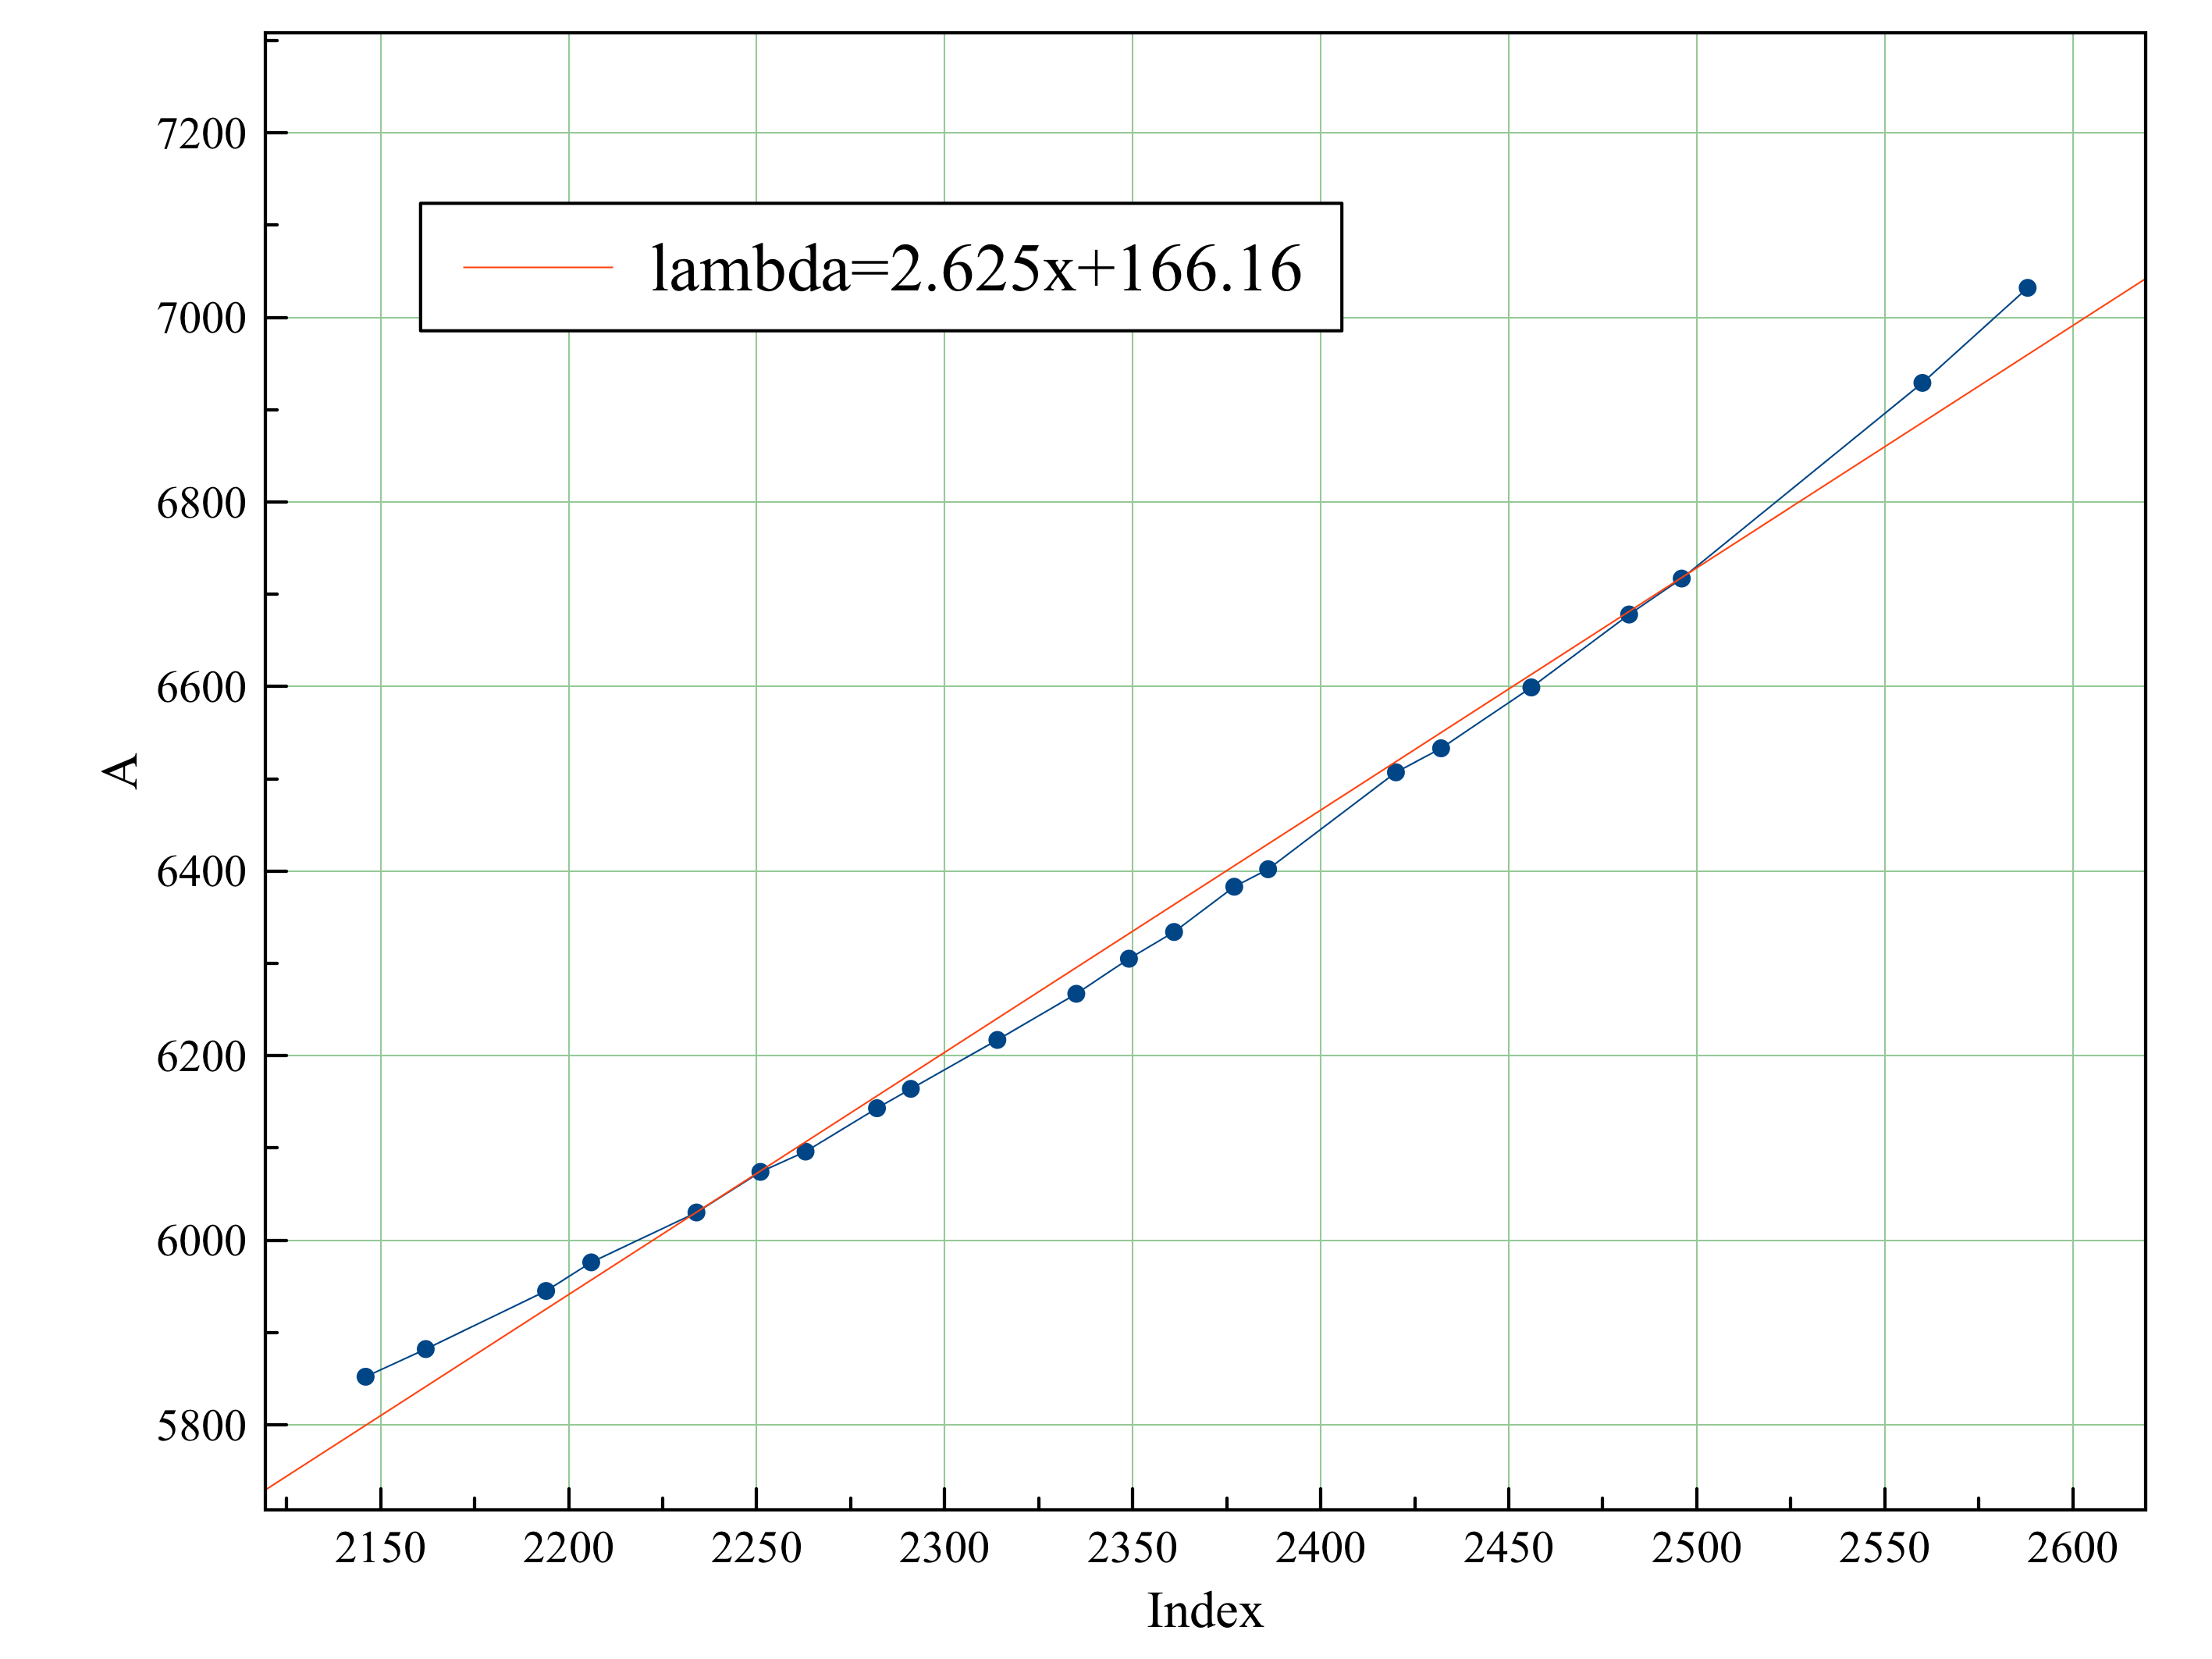
\includegraphics[width = 0.7\linewidth]{grad}
			\end{center}
			Теперь непосредственно снимем зависимости в координатах $(\sqrt{I}, V)$ и, экстраполируя данные, найдем запирающие напряжения из сделанных графиков
		
			Для каждого графика мы знаем точку пересечения с прямой $I = 0$, то есть запирающее напряжение, построим график $V_0$ от $w$ и найдем постоянную Планка. ($w=2\pi c/\lambda$, $\lambda$ находим из калибровочного графика, подставляя значение x, полученное в работе)
			\begin{center}
				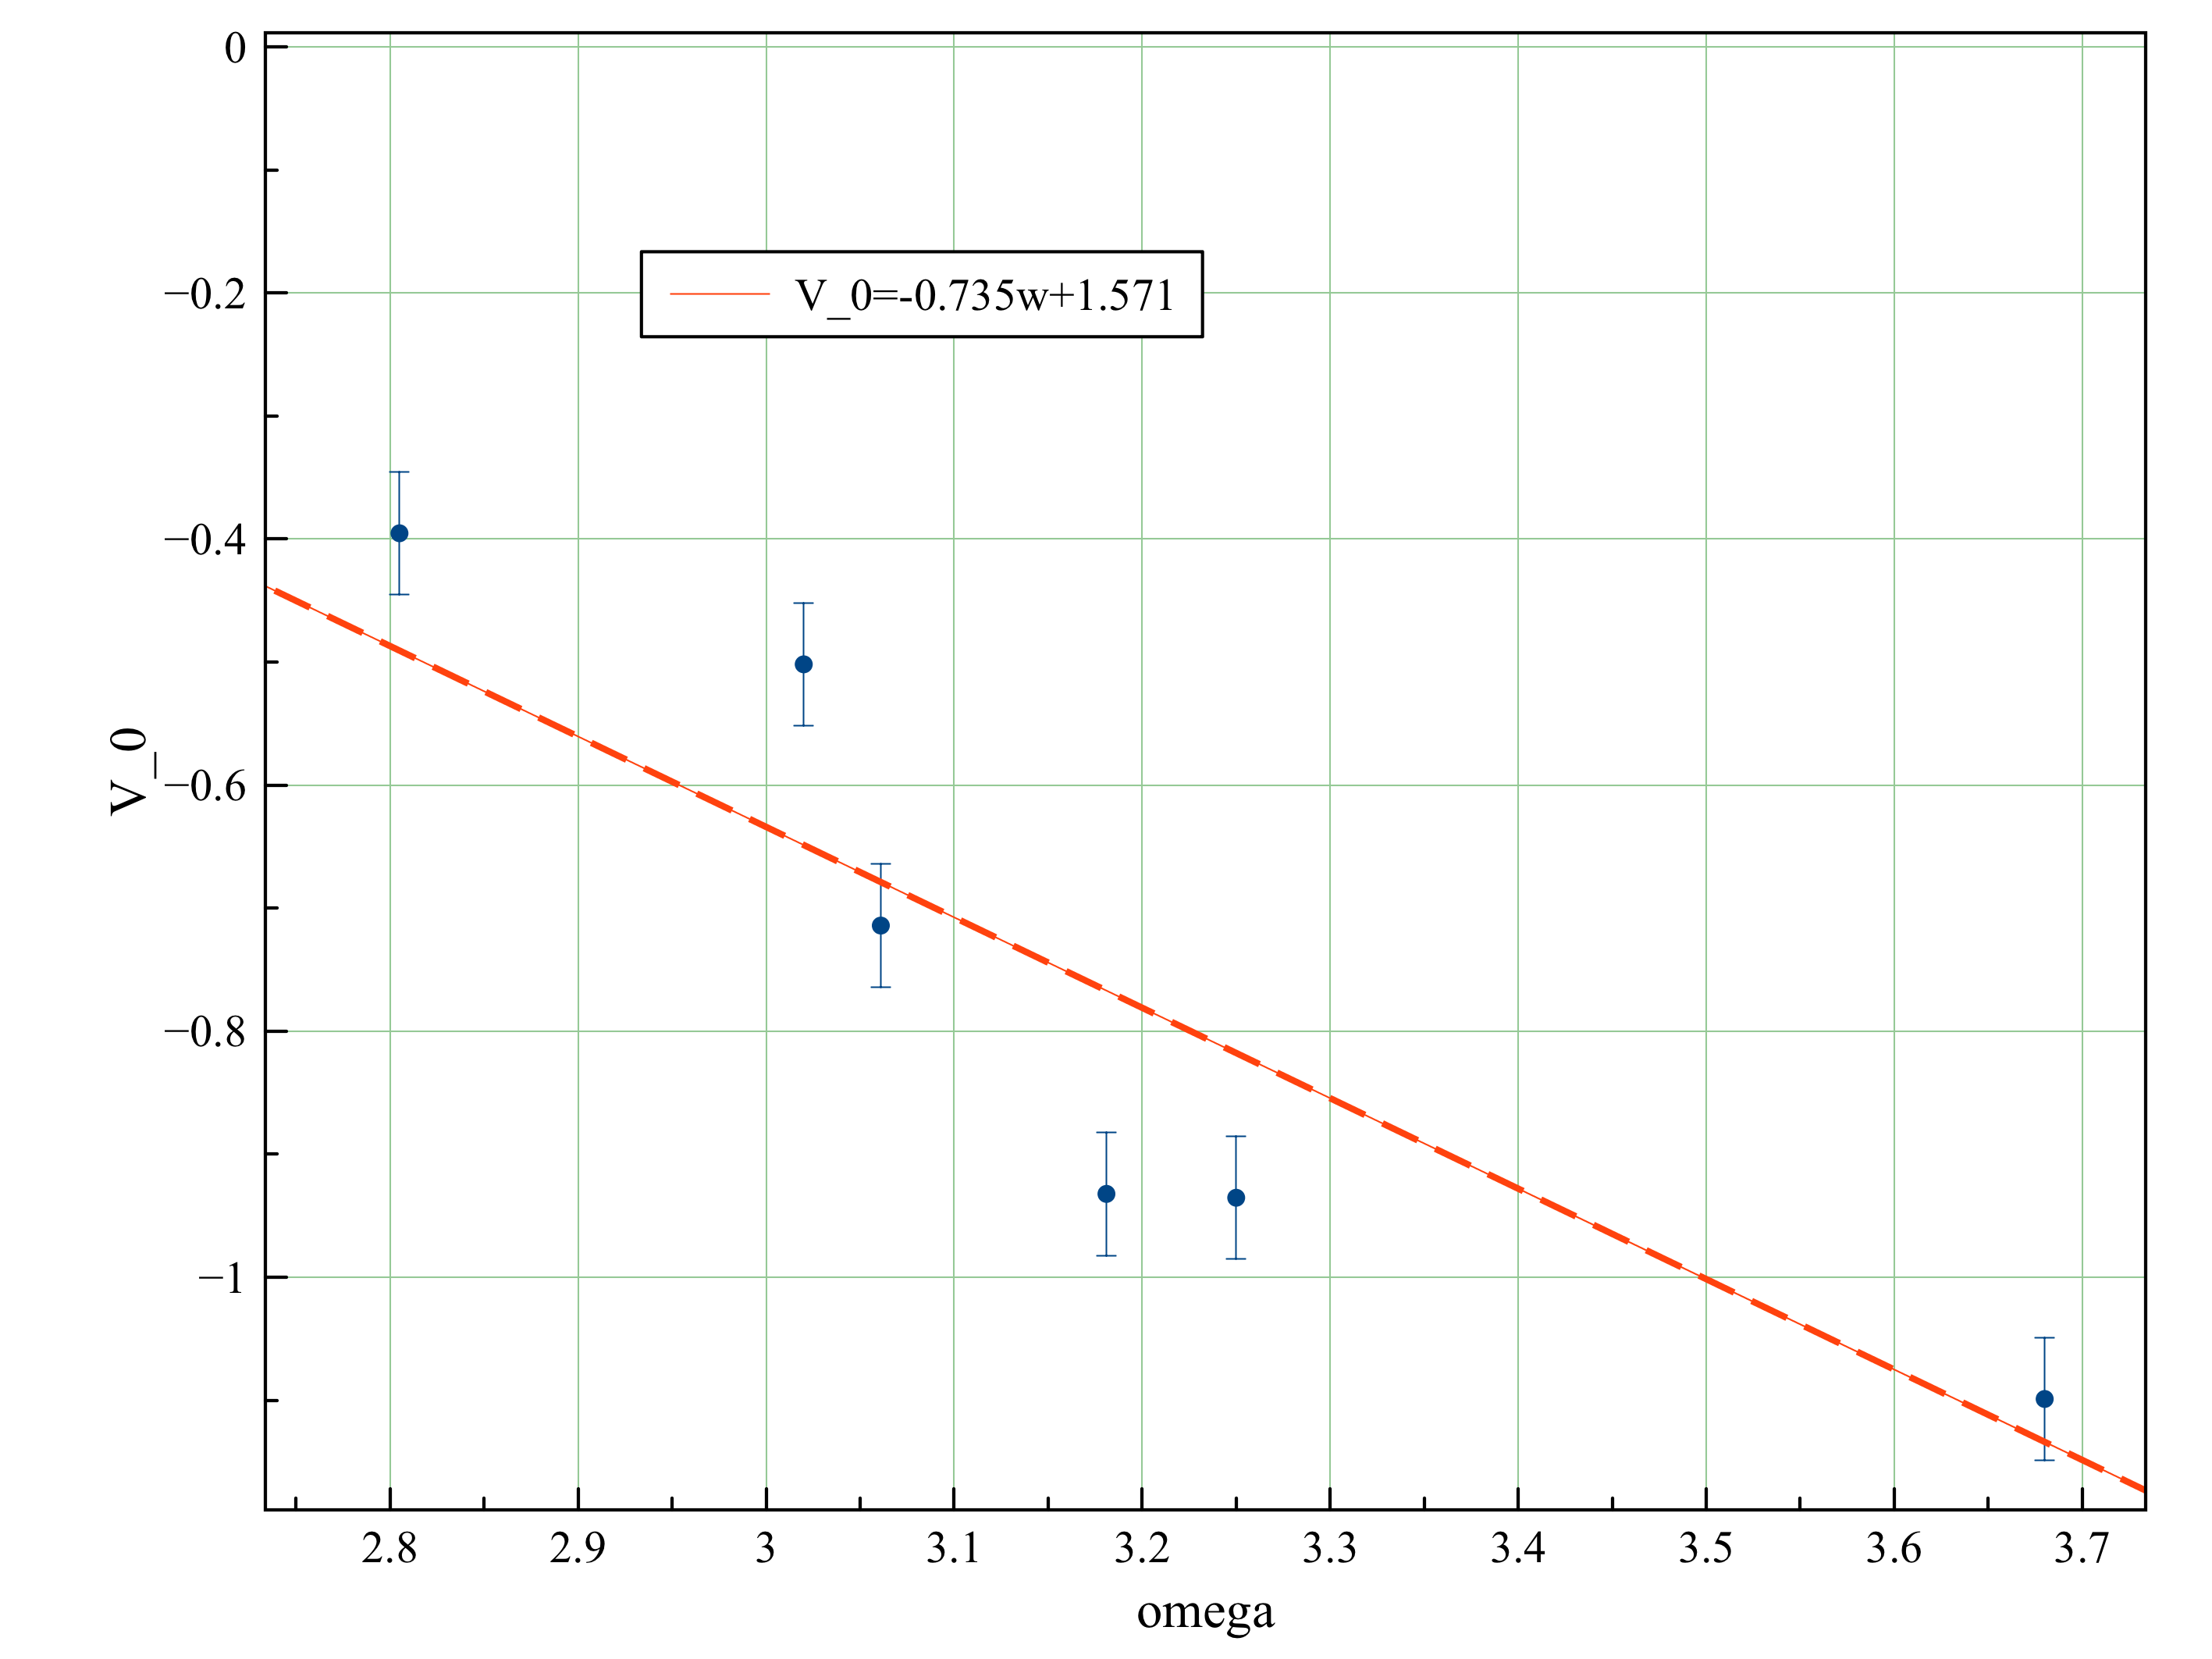
\includegraphics[width = 0.7\linewidth]{main}
			\end{center}
				\begin{center}
					\begin{figure}
						\centering
						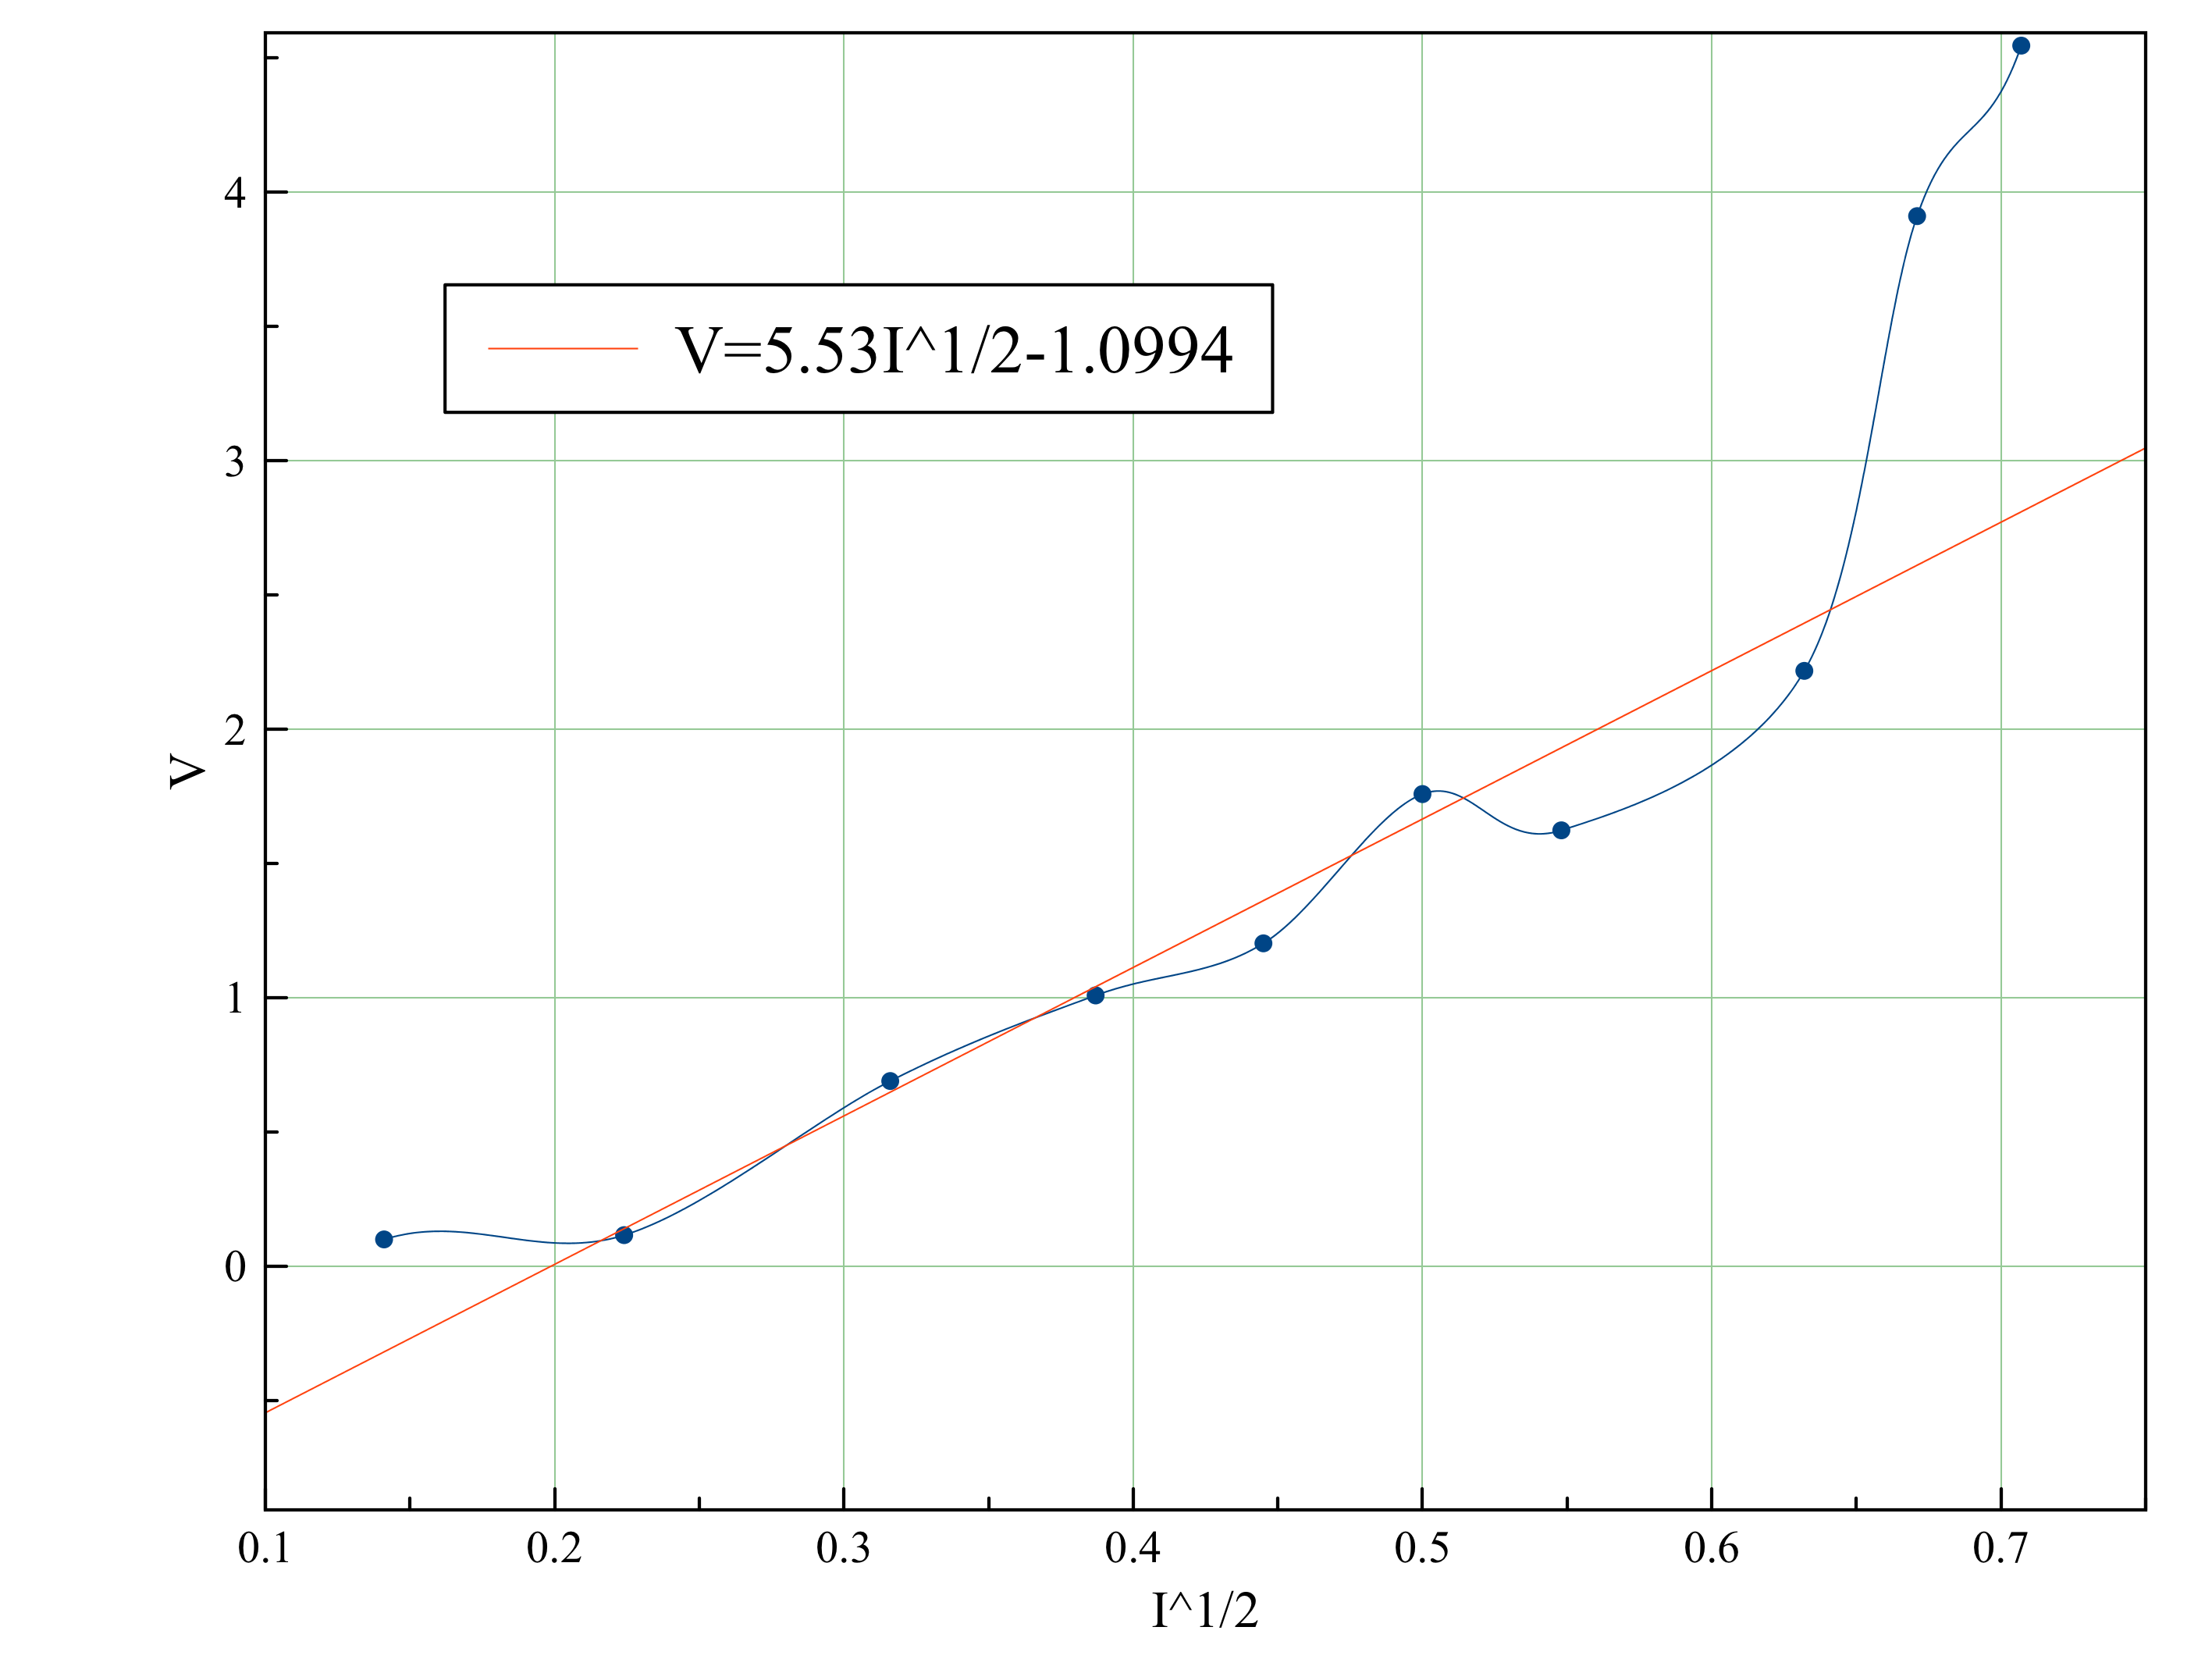
\includegraphics[width=0.6\linewidth]{1886}
						\caption{511,69 нм}
						
						\centering
						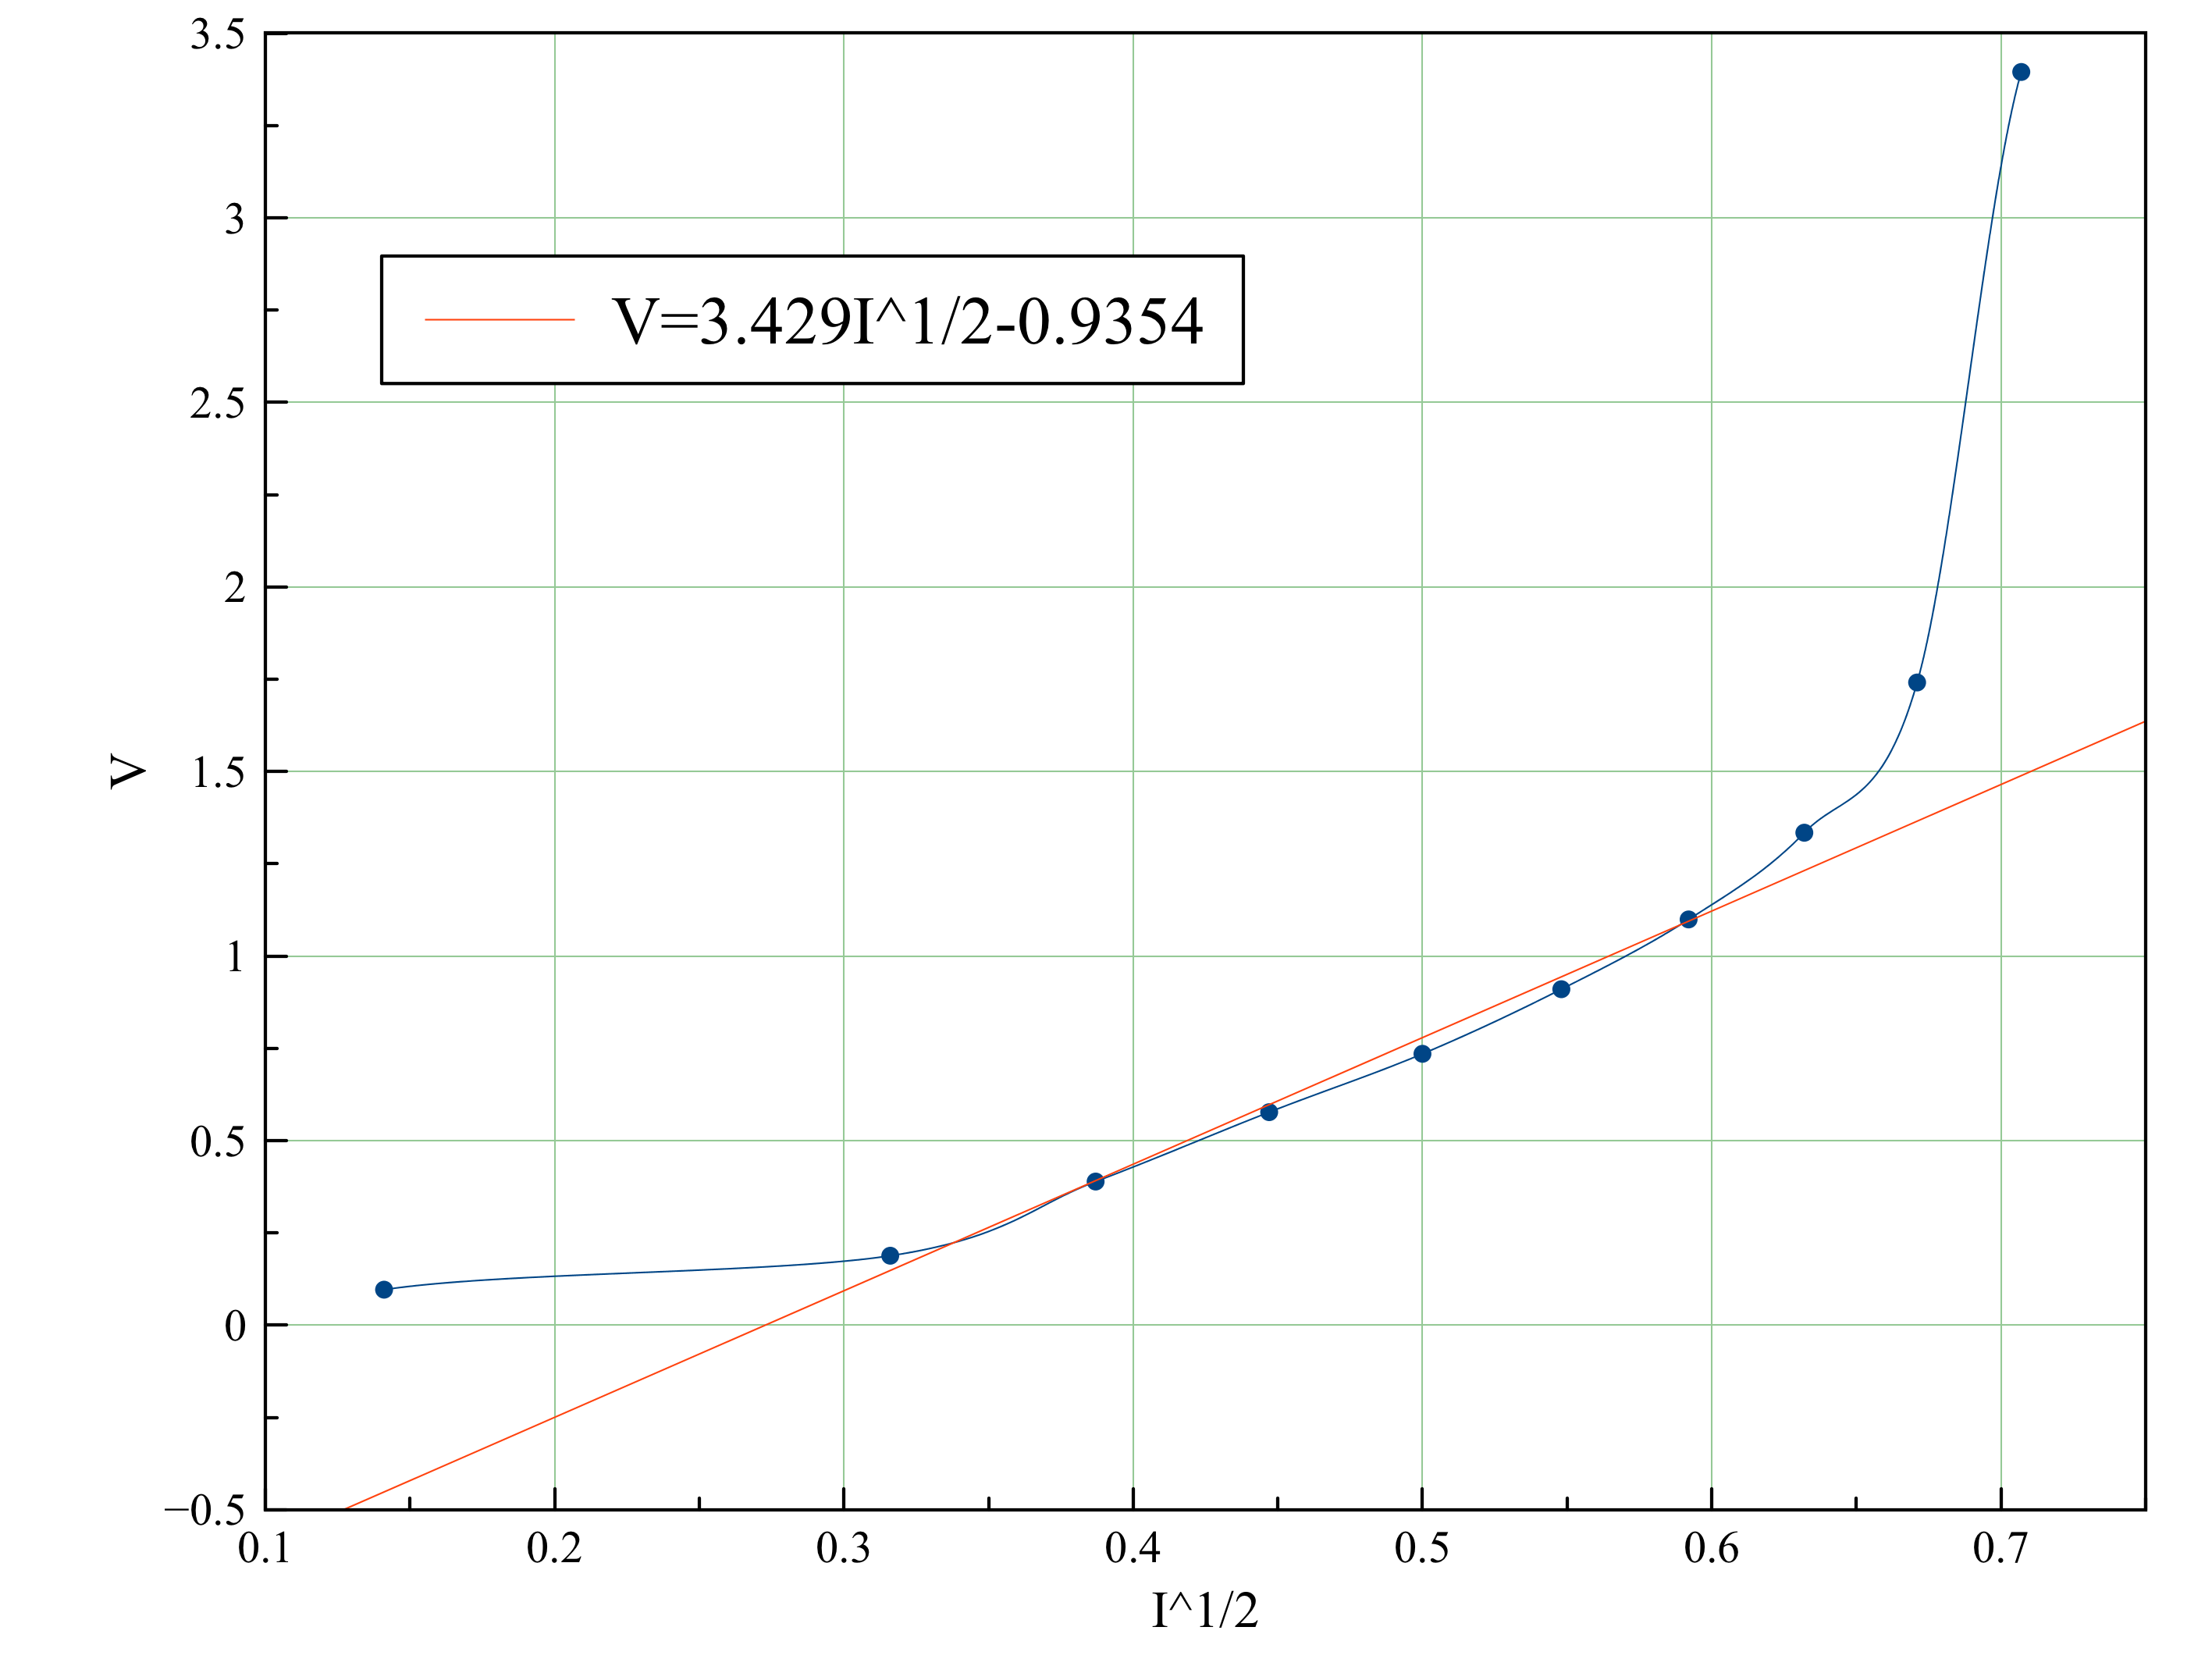
\includegraphics[width=0.6\linewidth]{2146}
						\caption{579,94 нм}
						
						\centering
						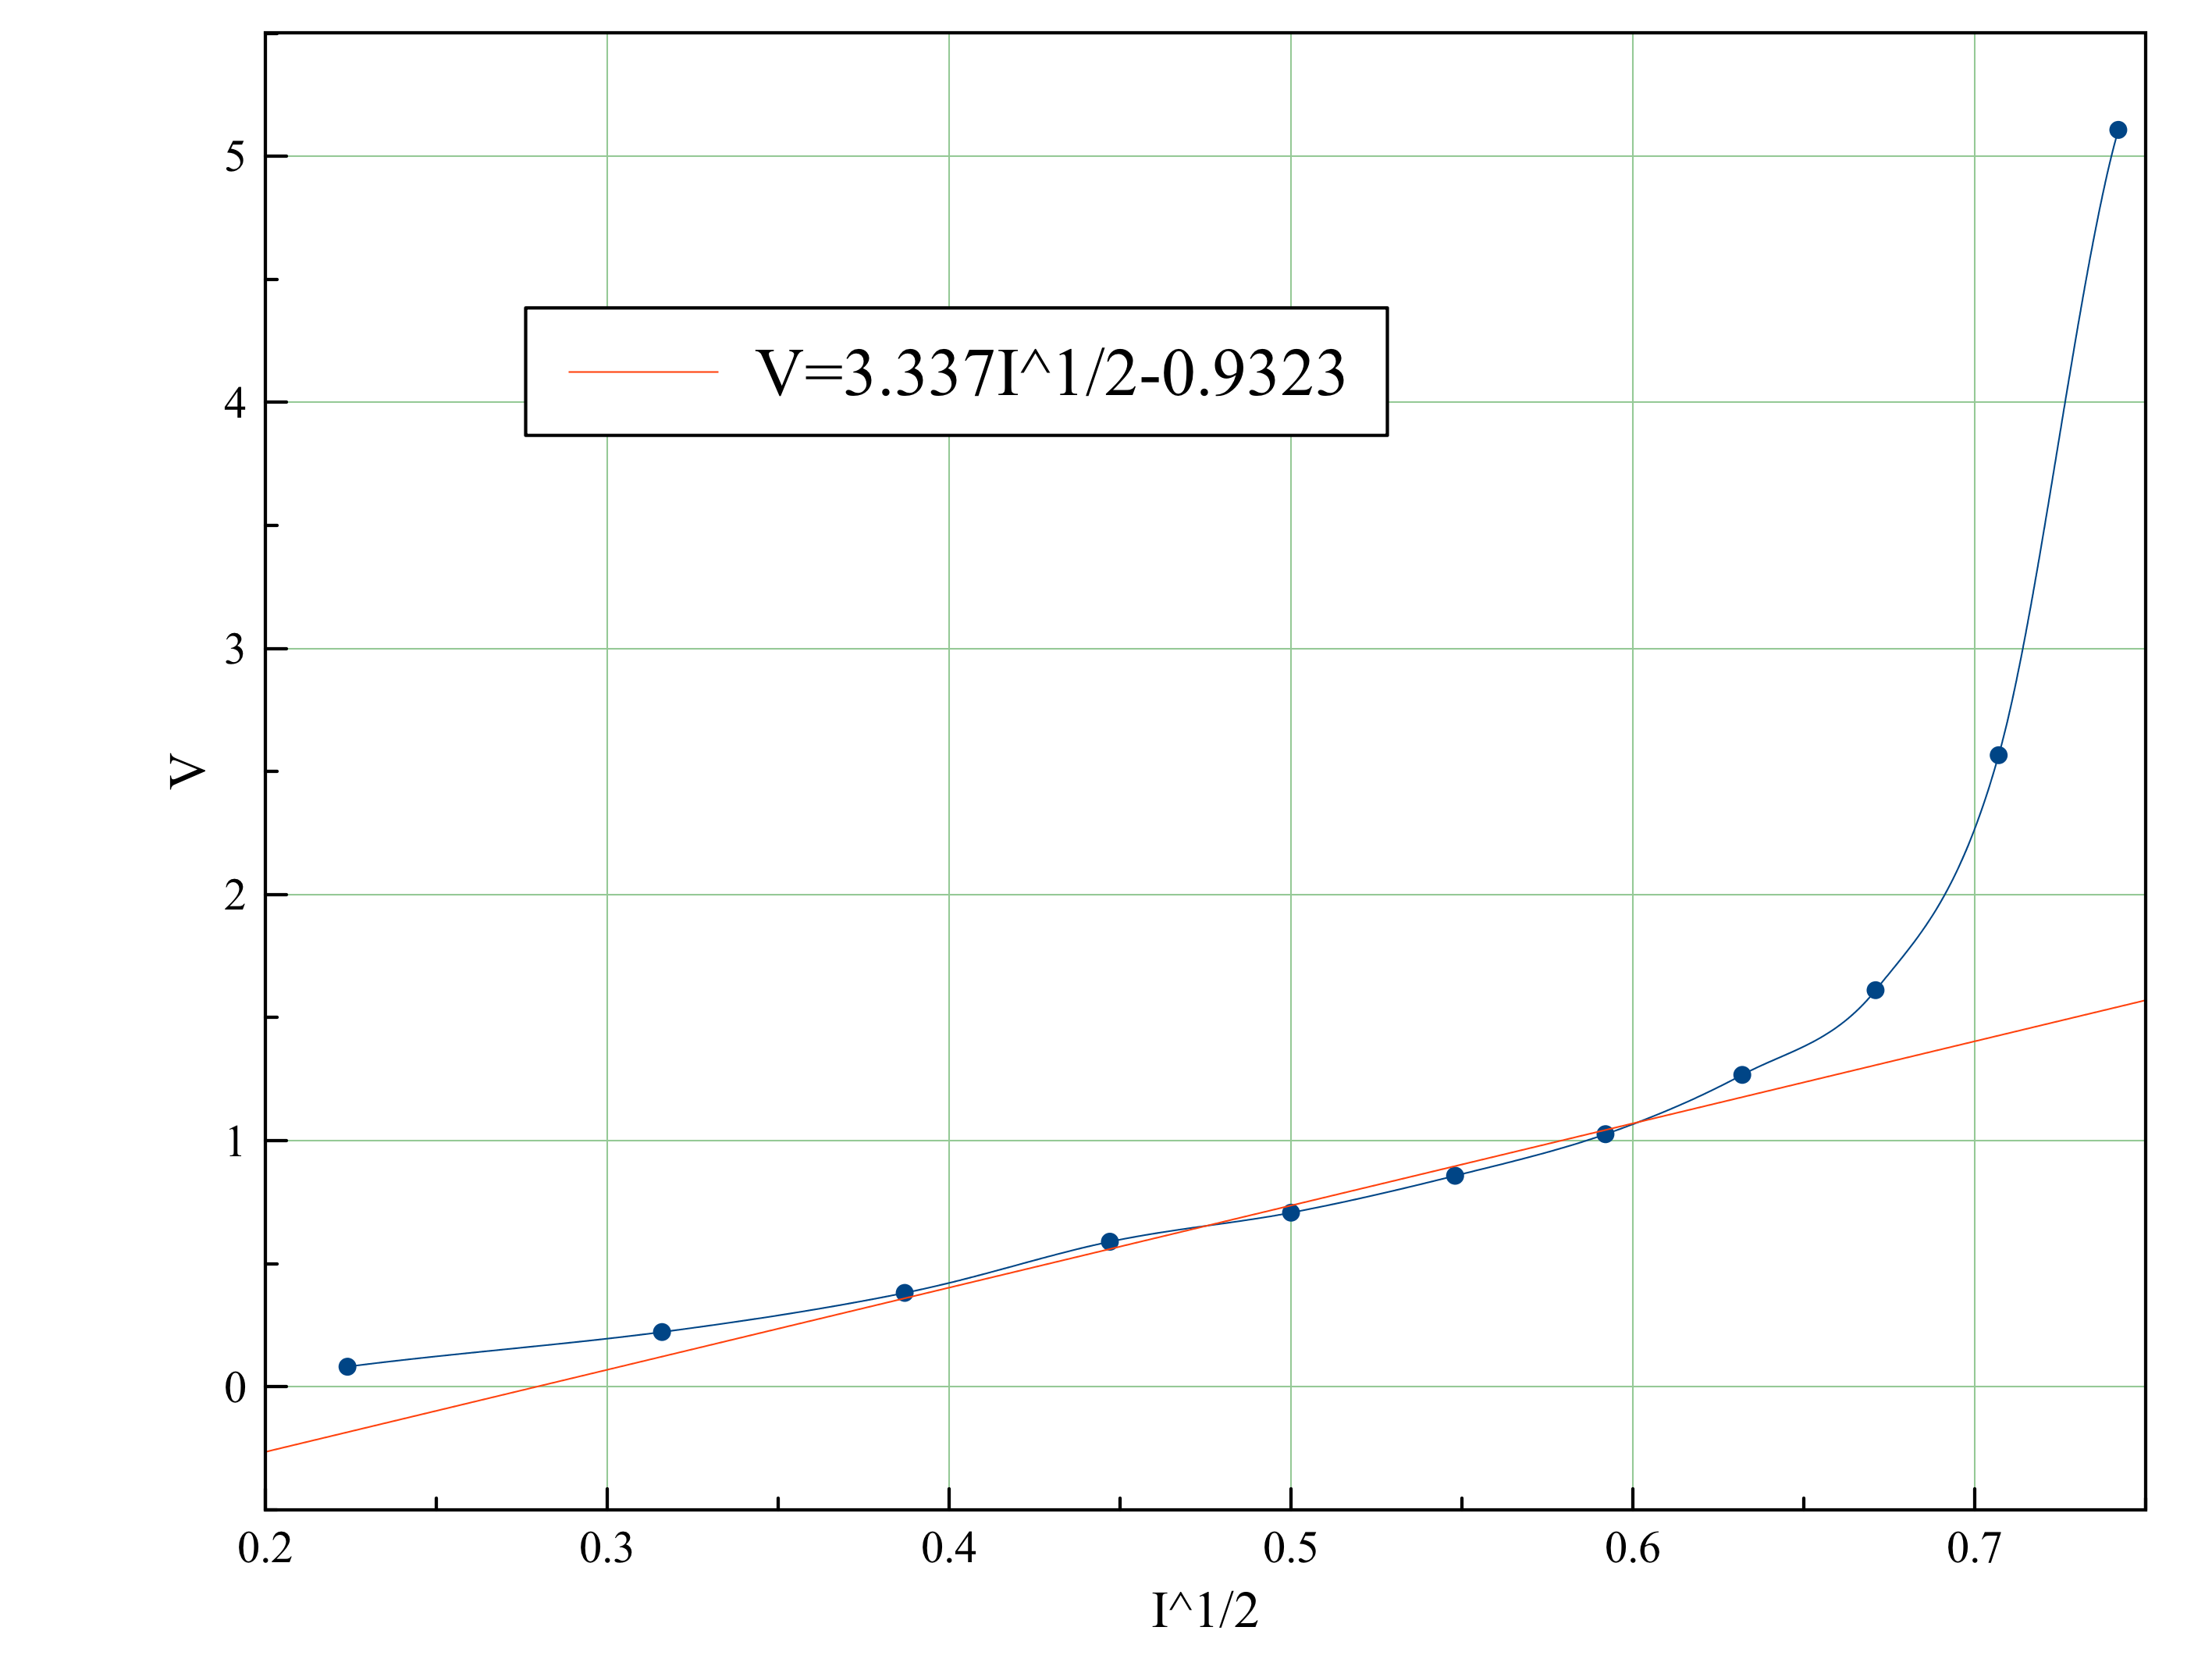
\includegraphics[width=0.6\linewidth]{2194}
						\caption{592,54 нм}
					\end{figure}
					\begin{figure}
						\centering
						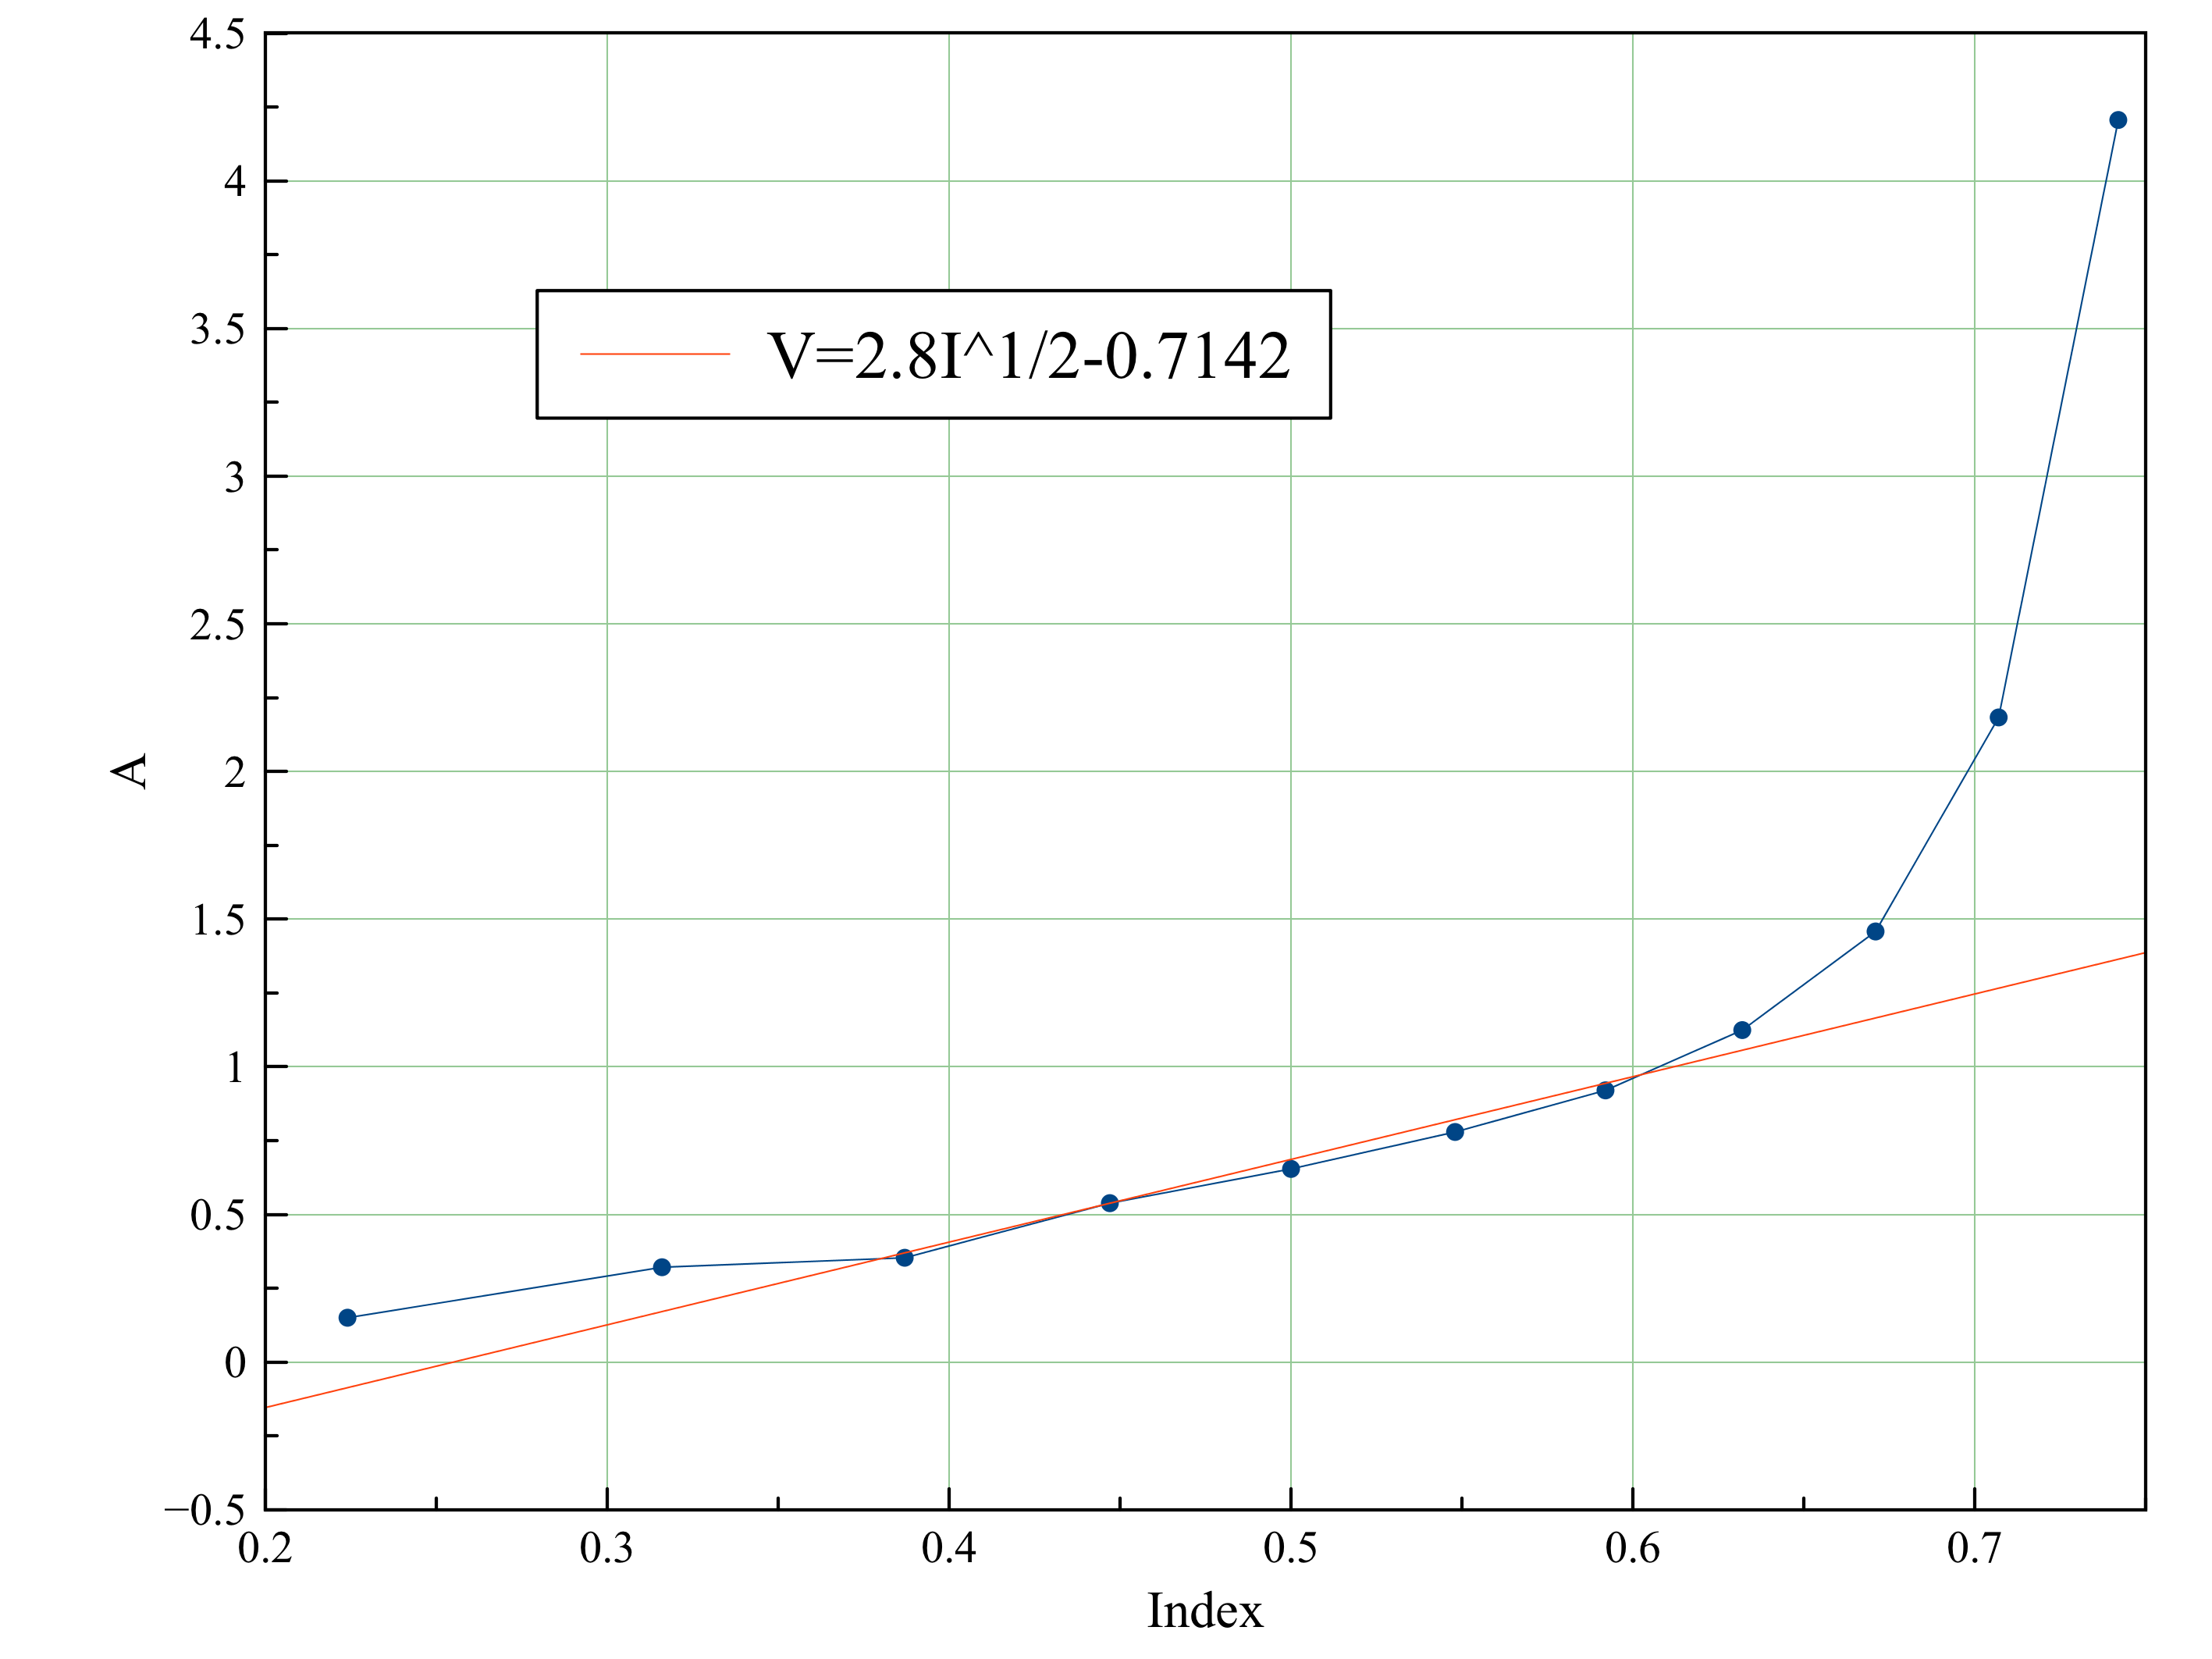
\includegraphics[width=0.6\linewidth]{2282}
						\caption{615,64 нм}
						
						\centering
						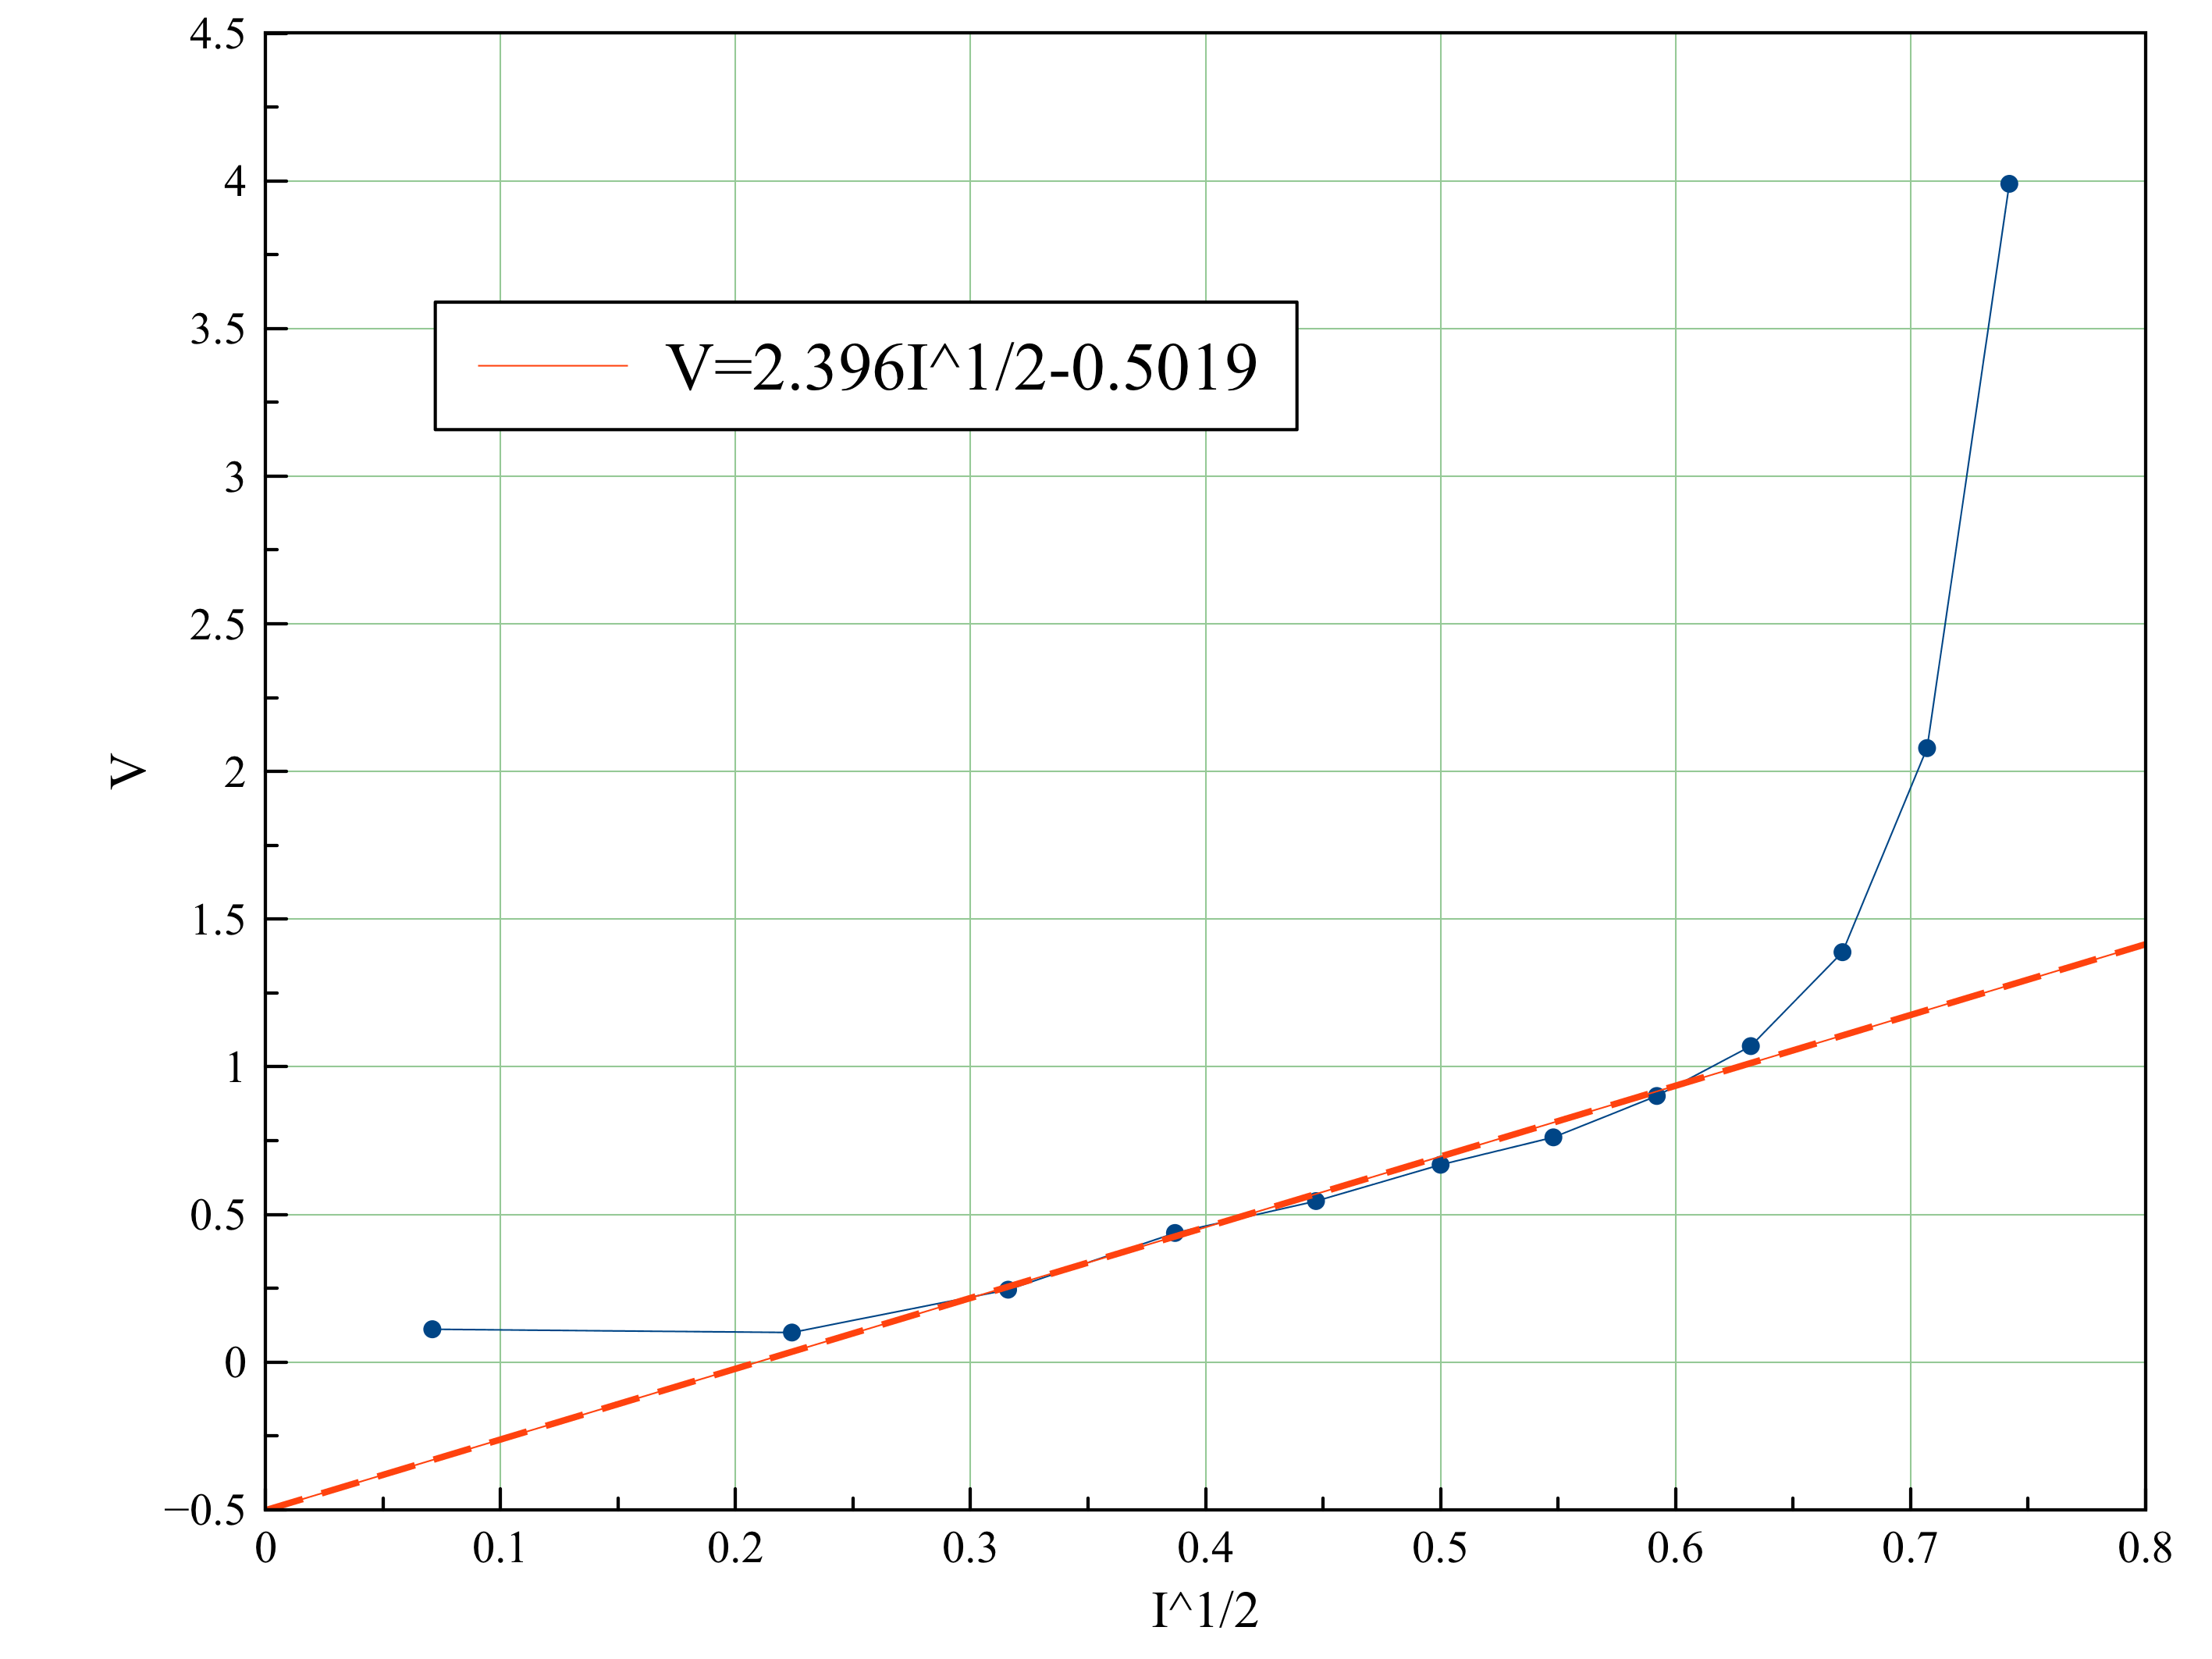
\includegraphics[width=0.6\linewidth]{2314}
						\caption{624,04 нам}
						
						\centering
						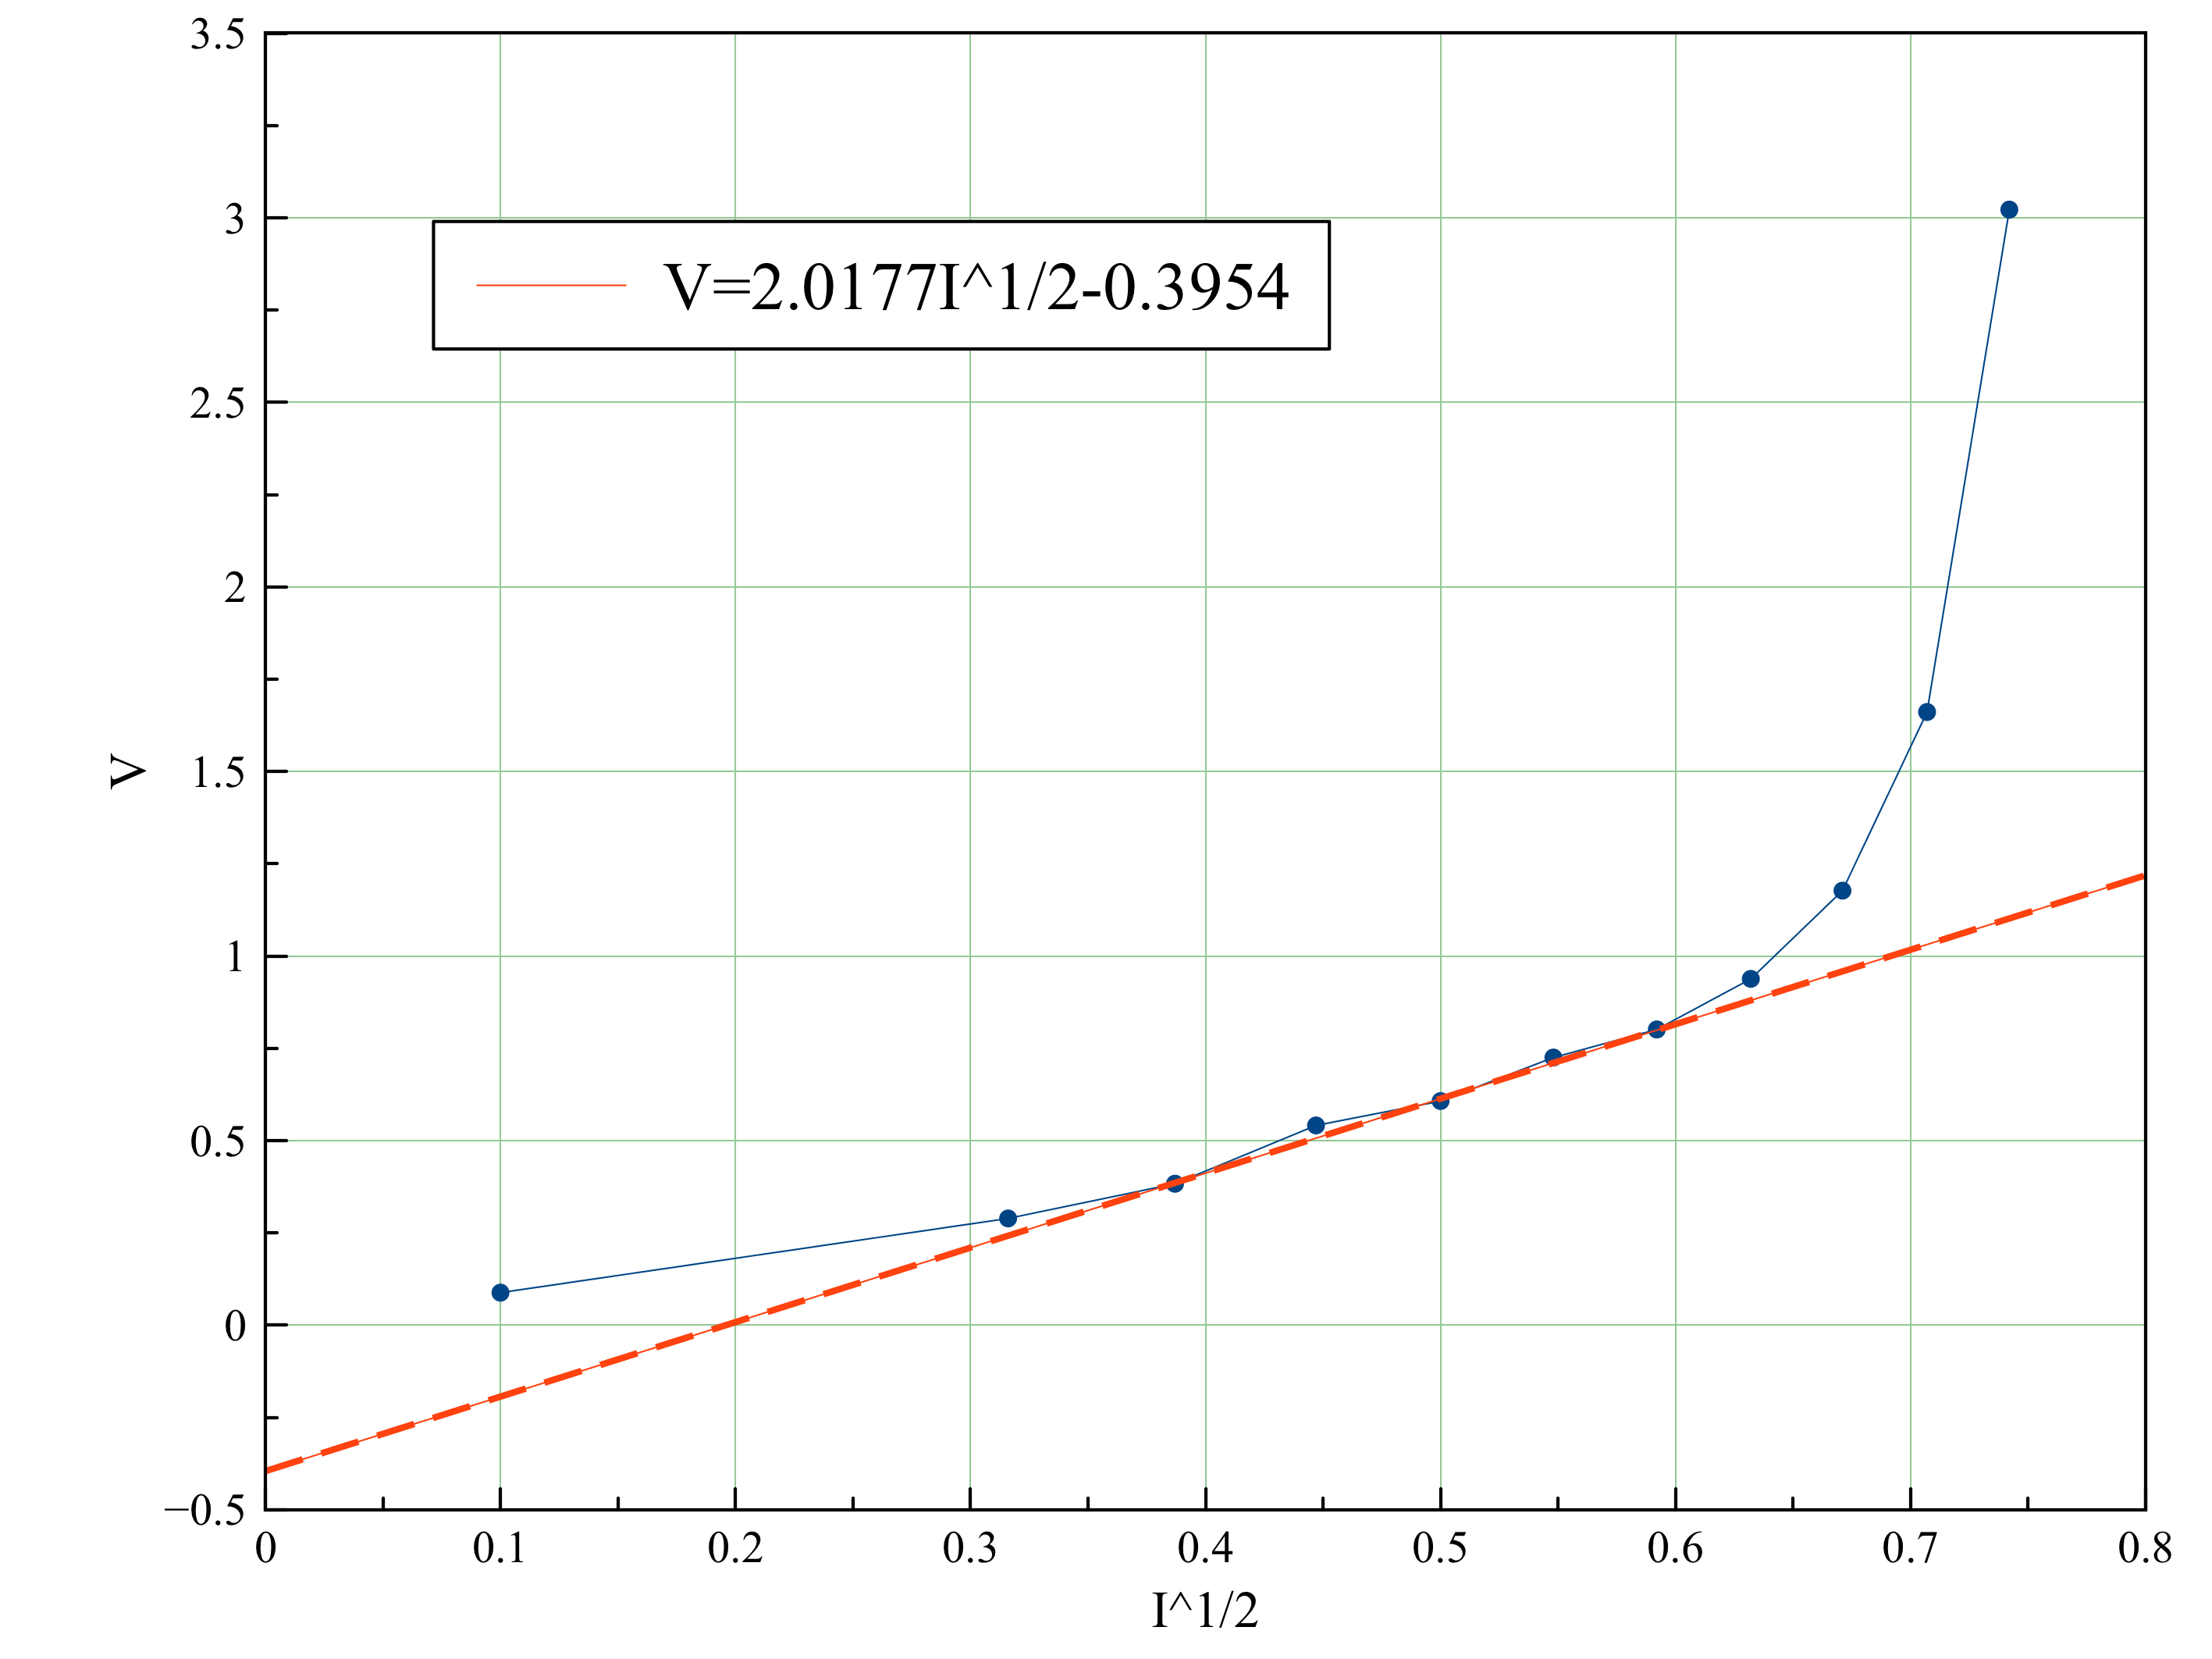
\includegraphics[width=0.6\linewidth]{2496}
						\caption{671,8 нм}
					\end{figure}
				\end{center}
			Методом наименьших квадратов найдем угловой коэффициент: $$b = \dfrac{dV_0}{dw} = 0.735  * 10^{-15} \text{В * сек}$$
			\textbf{Получаем по формуле $\dfrac{dV_0}{d\omega} = \dfrac{\hbar}{e}$, что постоянная планка равна: $$\hbar = 1.17 * 10 ^{-34} \text{Дж * сек}.$$}
			Мы получили довольно точную оценку, так как табличное значение равно $1.054* 10 ^{-34} \text{Дж * сек}.$
			
			
	\section*{Вывод}
	В данной работе провели исследование зависимости фототока от величины задерживающего потенциала и частоты падающего излучения. По ним вычислили величину постоянной Планка. Итоговый результат очень близкий к табличному значению. Таким образом, экспериментально проверили равнение Эйнштейна для фотоэффекта 

	

	
\end{document}
